\chapter{Modeling Automotive Systems}

With reference to three phase modeling approach described in section \ref{Sec_ThreePhaseModeling} consider modeling of following systems.

\section{Longitudinal vehicle dynamics model} \label{Sec_LongitudinalVehicleModel}

\textbf{\textit{Phase I}}: The whole of the vehicle can be treated as subsystem of following with respective inputs and outputs
\begin{enumerate}
	\item Powertrain \{ Pedal position -- Wheel traction forces \}
	\item Chassis \{ Wheel traction forces -- Vehicle velocity \}
	\begin{figure}[h!]
		\centering
		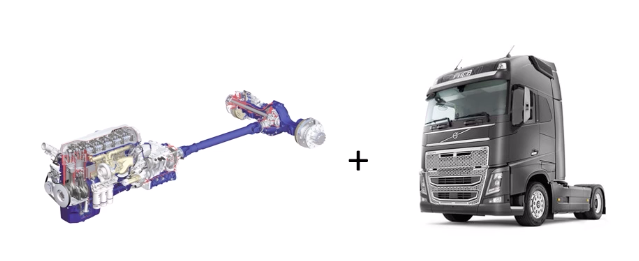
\includegraphics[width=0.5\linewidth]{Bilder/ModelAutoSystems_Subs1}
		\caption{Subsystems of entire vehicle model}
	\end{figure}
\end{enumerate}

In order to reduce modeling complexity, the above system can be further reduced into following subsystems
\begin{enumerate}
	\item Powertrain \{ Pedal position -- Wheel traction forces \}
	\begin{figure}[h!]
		\centering
		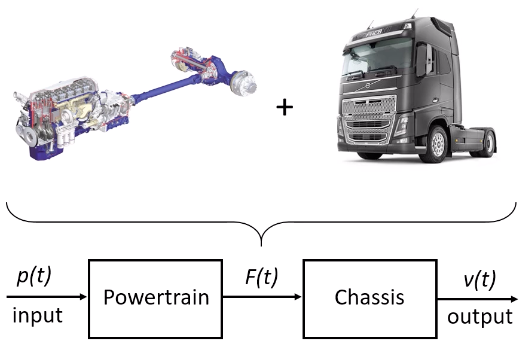
\includegraphics[width=0.5\linewidth]{Bilder/ModelAutoSystems_Subs2}
		\caption{Subsystems of entire vehicle model}
	\end{figure}
	\begin{enumerate}
		\item Engine \{ Pedal position -- Engine torque \}
		\item Gear box \{Engine Torque -- Gear box torque\}
		\item Wheel \{ Gear box torque -- Wheel traction forces \}
		\begin{figure}[h!]
			\centering
			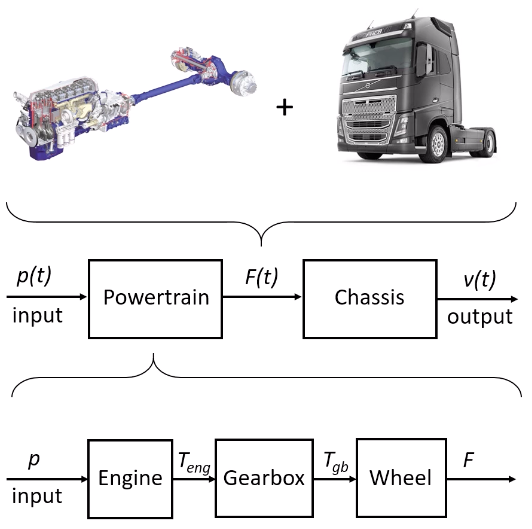
\includegraphics[width=0.5\linewidth]{Bilder/ModelAutoSystems_Subs3}
			\caption{Further Subsystems of vehicle model}
		\end{figure}
	\end{enumerate}
	\item Chassis \{ Wheel traction forces -- Vehicle velocity \}
\end{enumerate}
\newpage

\textbf{\textit{Phase II}}: The following mathematical models for following subsystems are required
\begin{enumerate}
	\item Engine
	\item Gearbox
	\item Wheel
	\item Chassis
\end{enumerate}
For modeling engine, an assumption (approximation) is made such that the engine torque developed can be expressed using first order system response as
\begin{equation} \label{Eq_ModelAutoSysEngineModel}
	\dot{T_{eng}} = -\frac{1}{\tau} T_{eng} + \frac{K}{\tau} u
\end{equation}
where, $\tau$ is time-constant of frist order systems, $K$ is system gain and $u$ is system input. 

The gearbox model is assumed to be a fixed gear ratio model with gear ratio $i$
\begin{equation} \label{Eq_ModelAutoSysGBModel}
	T_{gb} = i T_{eng}
\end{equation}
The wheel model converts the torques to ground traction forces
\begin{equation}
	F = \frac{T_{gb}}{r_{w}}
\end{equation}
which can be further expressed using equations \eqref{Eq_ModelAutoSysEngineModel} and \eqref{Eq_ModelAutoSysGBModel}
\begin{equation} \label{Eq_ModelAutoSysWheel}
	\dot{F} = -\frac{1}{\tau} F + \frac{K i}{\tau r_w} u
\end{equation}

For modeling the chassis, conservation laws can be used from Newton's
\begin{equation}
	\sum_{i}^{} F_i = m a
\end{equation}
further using free body diagram
\begin{figure}[h!]
	\centering
	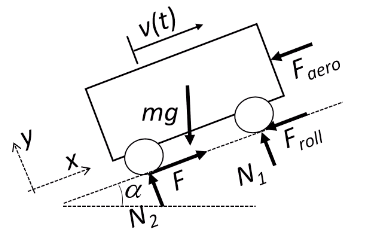
\includegraphics[width=0.5\linewidth]{Bilder/ModelAutoSystems_FBD}
	\caption{Free body diagram chassis model}
\end{figure}
using FBD, the following model can be expressed
\begin{align}
	x: m a &= F - F_{roll} - F_{Aero} - F_{grad} \label{Eq_ModelAutoSysFBDx} \\
	y: 0 &= N_{1} + N_{2} - m g cos\alpha
\end{align}
Using constitutive relationships
\begin{align}
	a &= \frac{dv}{dt} \\
	F_{roll} &= m g f cos\alpha \\
	F_{Aero} &= 0.5 \rho C_{d} A_{f} v^2 \\
	F_{grad} &= m g sin\alpha
\end{align}

\textbf{\textit{Phase III}}: From the equations developed in Phase II, it can be seen that there is a time derivative term for velocity and force has time derivatives associated with them. So choosing $F$ and $v$ as the state variables (There is another constitutive relationship $v = dy/dt$, but here the output will be written in terms of $v$ which will be the required state space. Therefore, ignoring this state variable)

From the states chosen writing the state-space model. Start from $F$ using equation \eqref{Eq_ModelAutoSysWheel}
\begin{equation}
	\frac{dF}{dt} = -\frac{1}{\tau} F + \frac{K i}{\tau r_w} u
\end{equation}
this equation is already in the form $\dot{x} = f(x,u,d)$. Further for state $v$, using equation \eqref{Eq_ModelAutoSysFBDx}
\begin{equation}
	m a = F - F_{roll} - F_{Aero} - F_{grad}
\end{equation}
the above equation is not in the form $\dot{x} = f(x,u,d)$, therefore using constitutive relations expressed in phase II
\begin{equation}
	\frac{dv}{dt} = \frac{1}{m} \left\{F - m g f cos\alpha -0.5 \rho C_{d} A_{f} v^2 - m g sin\alpha \right\}
\end{equation}
the above equation is now in the form $\dot{x} = f(x,u,d)$, this completes the state-space model. Further for the sake of simplicity new variable names can be used (entirely optional step)
\begin{align}
	x_1 &= F \\
	x_2 &= v
\end{align}
which leads to
\begin{align}
	\dot{x_1} &= -\frac{1}{\tau} x_1 + \frac{K i}{\tau r_w} u \\
	\dot{x_2} &= \frac{1}{m} \left\{x_1 - m g f cos\alpha -0.5 \rho C_{d} A_{f} {x_2}^2 - m g sin\alpha \right\}
\end{align}

\section{Modeling Drivetrain}

The simplified drivetrain model as described in section \ref{Sec_LongitudinalVehicleModel} considers the entire drive train dynamics as a first order response to the step control input. This model could be used in case when simulating vehicle scenarios at higher speeds. At lower speeds when the engine torque is high, the drive shaft and gear box shafts gets twisted and due to this oscillations are generally observed in the torque transmitting driveshaft. A controller can be used to avoid these oscillations so that a smooth torque be delivered to wheel shaft. In order to do so firstly, a model describing this dynamic behavior is captured used Modeling techniques in more detail.

Following the three phase modeling method as described in section \ref{Sec_ThreePhaseModeling},

\subsection{Phase I}: Since a more detailed dynamics of the system is now required to be captured, a subsystem model is now more detailed with most of the dynamic parts included into separate subsystems as shown in figure \ref{Fig_ModelingAutoSys_Drivetrain_1}
\begin{figure}[h!]
	\centering
	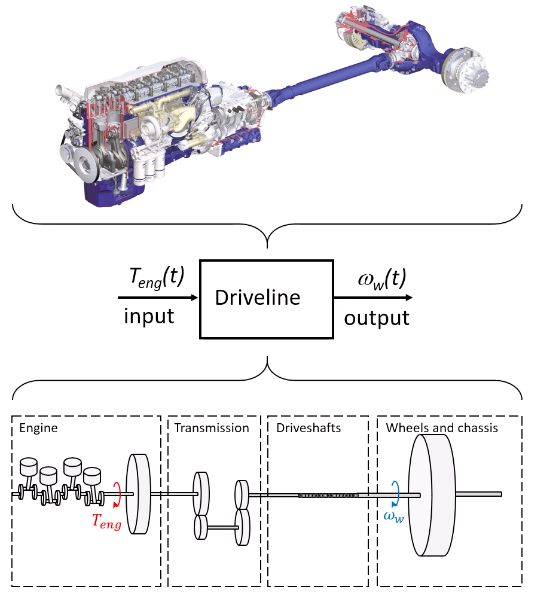
\includegraphics[width=0.6\linewidth]{Bilder/ModelingAutoSys_Drivetrain_1}
	\caption{Detailed subsystems of drivetrain}
	\label{Fig_ModelingAutoSys_Drivetrain_1}
\end{figure}
This is a rotatory system, therefore, Newton's law on rotating bodies is used. Using equation of angular momentum as expressed in Prelims in equation \eqref{Eq_Prelims_AngularMometumMatrixForm}, the sum total of all the torques acting on the subsystem is expressed as the time-derivative of equation \eqref{Eq_Prelims_AngularMometumMatrixForm}.
\begin{equation}
	\sum_{i}^{} \mathcal{T} = \vec{I} \dot{\omega}
\end{equation}
The term from $\vec{v_{A/O}} \times \vec{P_{/O}}$ equation \eqref{Eq_Prelims_AngularMometumMatrixForm} goes to zero as the distance vector $\vec{v_{A/O}} = 0$ or both the vectors $\vec{v_{A/O}}$ and $\vec{P_{/O}}$ are parallel.

\subsection{Phase II}: Drawing FBD's for the drivetrain subsystem given in figure \ref{Fig_ModelingAutoSys_Drivetrain_1} as shown in figure \ref{Fig_ModelingAutoSys_Drivetrain_2}
\begin{figure}[h!]
	\centering
	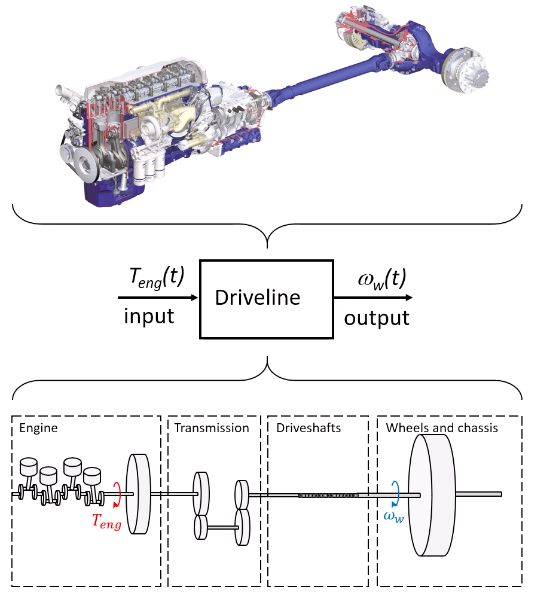
\includegraphics[width=\linewidth]{Bilder/ModelingAutoSys_Drivetrain_1}
	\caption{FBD of subsystems of drivetrain}
	\label{Fig_ModelingAutoSys_Drivetrain_2}
\end{figure}
While connecting these subsystems the following internal variables indicated in red comes to picture, also consider the following assumptions that are made for simplification
\begin{enumerate}
	\item Subsystem Engine: Inertia is modeled for the flywheel
	\item Subsystem Transmission: Inertia is considered negligible and subsystem is modeled as gear ratio between engine shaft and the transmission shaft
	\item Subsystem Driveshaft: Again inertia is neglected and subsystem is modeled as spring-damper system in parallel in order to include the first order dynamics of the shaft for an input torque
	\item Subsystem Wheels: Inertia is modeled as a lumped parameter
	\item The load at the end $T_{load}$ can be determined using Longitudinal model (reverse dynamics)
\end{enumerate}

\subsubsection{Equation for engine}
For the conservation law, there are two torques that are acting at the inertial flywheel, one from applied engine torque and one as resistance torque from the transmission. With no constitutive relationships (while ignoring friction)
\begin{equation}
	\vec{I}\dot{\omega} = T_{eng} - T_{tr1}
\end{equation}

\subsubsection{Equations for transmission}

The conservation law for transmission is simple as there is no inertia, the term $I \dot{\omega} = 0$. Therefore, the input torque should be equal to the output torque. Additionally, since the output torque gets multiplied by the transmission ratio, this should be included at the output torque
\begin{equation} \label{Eq_random_21}
	0 = T_{tr2} - i T_{tr1}
\end{equation}
the constitutive relation is the speed reduction from the gear
\begin{equation} \label{Eq_random_24}
	\omega_{eng} = i \omega_{tr}
\end{equation}

\subsubsection{Equations for drivetrain}

For the conservation law in this case, as there is no inertia element, this subsystem also does not add any additional torques a the output, so the input torque should be equal to the output torque
\begin{equation} \label{Eq_random_22}
	0 = T_{ds} - T_{tr2}
\end{equation}
the constitutive relationship for this subsystem describes how the output torque changes dynamically due to spring-damper system like behavior of drivetrain
\begin{equation} \label{Eq_random_23}
	T_{ds} = c_s \left( \int (\omega_{tr} - \omega_{w}) dt \right) + d_s (\omega_{tr} - \omega_{w})
\end{equation}

\subsubsection{Equations for wheel and chassis}

The conservation law is again from Newtons law, here there is an inertia element, so there some dynamic loading of the output torque
\begin{equation}
	\vec{I_c}\dot{\omega_{w}} = T_{ds} - T_{load}
\end{equation}
the inertia term here has inertia due to wheels rotation and the inertia on the rotating mass due to the translating chassis, which is fixed to it
\begin{equation}
	\vec{I_c} = I_{wheel} + m r^{2}_{wheel}
\end{equation}
where $m$ is the mass of chassis

\subsection{Phase III}

In order to choose state variable, it can be seen from equations developed in phase II, there are two time-derivatives of $\omega_{eng}$ and $\omega_{w}$, further there is also an integral of these two components $\int (\omega_{tr} - \omega_{w}) dt$. This term is actually, the torsion of the drivetrain and called here $\varphi$. Therefore, 3 states variables have been identified.

Also note that the driveshaft torque can now be written as a function of torsion
\begin{equation}
	T_{ds} = c_s \varphi + d_s (\omega_{tr} - \omega_{w})
\end{equation}

Lets start from state $\omega{eng}$
\begin{equation}
	\dot{\omega_{eng}} = \frac{1}{I}(T_{eng} - T_{tr1})
\end{equation}
there is inputs in this equation but there are no state variables, using equation \eqref{Eq_random_21}
\begin{equation}
	\dot{\omega_{eng}} = \frac{1}{I}(T_{eng} - \frac{T_{r2}}{i} )
\end{equation}
continuing with equations \eqref{Eq_random_22} and \eqref{Eq_random_23}
\begin{equation}
	\dot{\omega_{eng}} = \frac{1}{I}(T_{eng} - \frac{1}{i}(c_s \varphi + d_s (\omega_{tr} - \omega_{w})))
\end{equation}
finally with equation \eqref{Eq_random_24}
\begin{equation}
	\dot{\omega_{eng}} = \frac{1}{I}(T_{eng} - \frac{1}{i}(c_s \varphi + d_s (\frac{\omega_{eng}}{i} - \omega_{w})))
\end{equation}
similarly, for state $\omega_{w}$
\begin{align*}
	\dot{\omega_{w}} &= \frac{1}{I_c} (T_{ds} - T_{load}) \\
					&= \frac{1}{I_c} (c_s \varphi + d_s (\omega_{tr} - \omega_{w}) - T_{load})
\end{align*}
\begin{equation}
	\dot{\omega_{w}} = \frac{1}{I_c} (c_s \varphi + d_s (\frac{\omega_{eng}}{i} - \omega_{w}) - T_{load})
\end{equation}

Finally, for state $\varphi$, the derivative is available directly
\begin{equation}
	\dot{\varphi} = \frac{\omega_{eng}}{i} - \omega_{w}
\end{equation}

the output is the wheel speed state variable
\begin{equation}
	y = \omega_{w}
\end{equation}

Optionally, the state-space model can be written using new variables $x_1 = \omega_{eng}$, $x_2 = \omega_{w}$ and $x_3 = \varphi$, load $T_{load}$ is considered a disturbance to the system
\begin{align}
	\dot{x_1} &= \frac{1}{I}(u - \frac{1}{i}(c_s \varphi + d_s (\frac{x_1}{i} - x_2))) \\
	\dot{x_2} &= \frac{1}{I_c} (c_s \varphi + d_s (\frac{x_1}{i} - x_2) - d) \\
	\dot{x_3} &= \frac{x_1}{i} - x_2
\end{align}

The above state-space form is linear, therefore it can written in matrix form
\begin{align}
	\dot{x} &= Ax + Bu + Hd \\
	y &= Cx + Du
\end{align}

\begin{align}
	\begin{bmatrix}
	\dot{x_1} \\ \dot{x_2} \\ \dot{x_3}
	\end{bmatrix} &= \begin{bmatrix}
		\frac{-d_s}{I i^2} & \frac{d_s}{I i} & \frac{-c_s}{I i} \\
		\frac{d_s}{I_c i} & \frac{-d_s}{I_c} & \frac{c_s}{I_c} \\
		\frac{1}{i} & -1 & 0
	\end{bmatrix} \begin{bmatrix}
	x_1 \\ x_2 \\ x_3
	\end{bmatrix} + \begin{bmatrix}
		\frac{1}{I} \\ 0 \\ 0 \\ 0
	\end{bmatrix} u + \begin{bmatrix}
		0 \\ \frac{-1}{I_c} \\ 0
	\end{bmatrix} d \\
	y &= [0 \quad 1 \quad 0] \begin{bmatrix}
	x_1 \\ x_2 \\ x_3
	\end{bmatrix} + [0]u
\end{align}

\section{Modeling suspension system}

\subsubsection{Phase I}
For modeling the suspension system, a quarter car model is used as shown in figure \ref{Fig_ModelAutoSys_SuspensionModel}
\begin{figure}[h!]
	\centering
	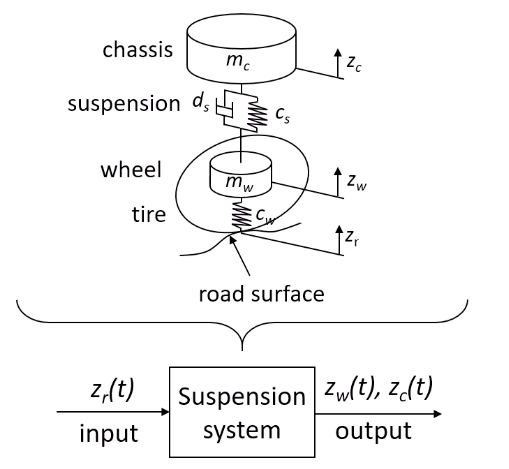
\includegraphics[width=0.6\linewidth]{Bilder/ModelAutoSys_SuspensionModel}
	\caption{Suspension model}
	\label{Fig_ModelAutoSys_SuspensionModel}
\end{figure}
\newpage

\subsubsection{Phase II}

Using FBD's as shwon in figure \ref{Fig_ModelAutoSys_SuspensionModel_FBD}
\begin{figure}[h!]
	\centering
	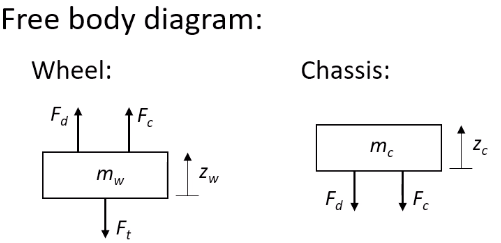
\includegraphics[width=0.75\linewidth]{Bilder/ModelAutoSys_SuspensionModel_FBD}
	\caption{Suspension model}
	\label{Fig_ModelAutoSys_SuspensionModel_FBD}
\end{figure}

For modeling wheel, using conservation law's (Newtons Law), a force balance can be used
\begin{equation}
	m_w a_w = F_c + F_d - F_t 
\end{equation}
For modeling chassis, again using conservation law on force balance
\begin{equation}
	m_c a_c = -F_d - F_c
\end{equation}

Constitutive relationships:
\begin{enumerate}
	\item \textbf{\textit{acceleration and velocity}}
	\begin{align}
		a_w &= \frac{d v_w}{dt} = \dot{v_w} \\
		a_c &= \frac{d v_c}{dt} = \dot{v_c} \\
		v_w &= \frac{d z_w}{dt} = \dot{z_w} \\
		v_c &= \frac{d z_c}{dt} = \dot{z_c} \\
	\end{align}
	\item \textbf{\textit{spring and damper elements -- using Hooke's law}}
	\begin{align}
		F_t &= c_w (z_w - z_r) \quad \text{Tire force} \\
		F_c &= c_s (z_c - z_w) \quad \text{Suspension spring} \\
		F_d &= d_s (v_c - v_w) \quad \text{Suspension damper} \\
	\end{align}
\end{enumerate} 

\subsubsection{Phase III}

From phase II it can be seen that there are four time derivatives, so choosing states as 
$$ \{ z_w, v_w, z_c, v_c \} $$ the state-space model can be expressed with new variables $$ \{ x_1 = z_w, x_2 = v_w, x_3 = z_c, x_4 = v_c  \} $$ as (the model is linear, so it can be written in the Matrix form)
\begin{align}
	\begin{bmatrix}
	\dot{x_1} \\\dot{x_2} \\ \dot{x_3} \\ \dot{x_4}
	\end{bmatrix} &= \begin{bmatrix}
		0 & 1 & 0 & 0 \\ 
		\frac{-(c_w + c_s)}{m_w} & \frac{-d_s}{m_w} & \frac{c_s}{m_w} & \frac{d_s}{m_w} \\
		0 & 0 & 0 & 1 \\
		\frac{c_s}{m_c} & \frac{d_s}{m_c} & \frac{-c_s}{m_c} & \frac{-d_s}{m_c}
	\end{bmatrix} \begin{bmatrix}
	x_1 \\ x_2 \\ x_3 \\ x_4
	\end{bmatrix} + \begin{bmatrix}
		0 \\ \frac{c_w}{m_w} \\ 0 \\ 0
	\end{bmatrix} u \\
	\begin{bmatrix}
		y_1 \\ y_2 \end{bmatrix} &= \begin{bmatrix}
			1 & 0 & 0 & 0 \\ 0 & 0 & 1 & 0
		\end{bmatrix}\begin{bmatrix}
		x_1 \\ x_2 \\ x_3 \\ x_4
		\end{bmatrix} + \begin{bmatrix}
			 0 & 0 
		\end{bmatrix} u	
\end{align}

If the dynamics of comfort is controlled by only designing the parameters of spring and damping of the suspension it is called \textbf{\textit{Passive Suspension}}, however, if an actuator is used to control the comfort dynamics against the disturbance from road then it is called \textbf{\textit{Active Suspension}}

\section{Single track vehicle model} \label{Sec_2_ch_26_SingleTrackModel}

This is the model required to control the motion of the vehicle. This model defines the lateral dynamics of the vehicle when it is steered. 

\subsection{Modeling assumptions}

\begin{enumerate}
	\item Only planar motion is considered ie., along x, y directions and orientation ${\psi}$
	\item Pitch, roll and vertical motions are not included, however, the vertical motion of the vehicle can be studied using the suspension model. For including pitch and roll an additional 2 DOF (about the pitch and roll axis) model has to be constructed.
\end{enumerate}

There are two kinds of planar motion models used to describe and control the vehicles motion
\begin{enumerate}
	\item Two track model (4 Wheeled vehicle model with steering and lateral dynamics)
	\item Single track model (Bicycle model)
	\begin{enumerate}
		\item Linear single track model
		\item Nonlinear bicycle model (nonlinear Tyre characteristics among others)
	\end{enumerate}
\end{enumerate}

\subsection{Phase I}

In single track model, the 4 wheeled vehicle model is limited to having one steerable wheel and one rear wheel. Since it is a lateral dynamic model, the model input is steering and output is the lateral motion described by $v_y$ and $\psi$ as shown in figure \ref{Fig_ModelAutoSys_SingleTrackModel}
\begin{figure}[h!]
	\centering
	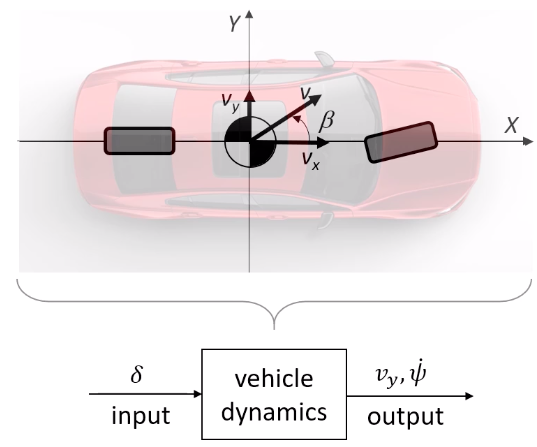
\includegraphics[width=0.65\linewidth]{Bilder/ModelAutoSys_SingleTrackMdoel}
	\caption{Single track model}
	\label{Fig_ModelAutoSys_SingleTrackModel}
\end{figure}
\newpage

\subsection{Phase II} \label{Sec_Phase2BicycleModel}

As this is a mechanical system, to describe the dynamics, consider the FBD as shown in figure \ref{Fig_ModelAutoSys_SingleTrackModel_FBD}
\begin{figure}[h!]
	\centering
	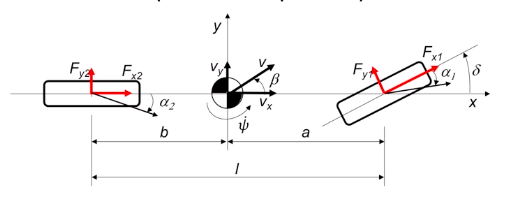
\includegraphics[width=\linewidth]{Bilder/ModelAutoSys_SingleTrackMdoel_FBD}
	\caption{Single track model}
	\label{Fig_ModelAutoSys_SingleTrackModel_FBD}
\end{figure}

$F_{i}$ are the longitudinal and lateral forces in the individual wheel frames. $\alpha_{1}$ and $\alpha_{2}$ are the front and rear wheel slip angles, i.e., the angles that the wheel propagation velocities make with the actual bicycles propagation (this is how the required centrifugal force develops). $\beta$ is the angle that the propagation velocity makes with the bicycles frame. Here, the component velocities $V_{x}$ and $V_{y}$ are in the bicycles frame, in the simplified case shown in figure \ref{Fig_ModelAutoSys_SingleTrackModel_FBD}, this is also the frame of the rear wheel. $\delta$ is the steering angle with reference to bicycles frame.

Additionally, also note that the lateral forces $F_{y1}$ and $F_{y2}$ shown in figure \ref{Fig_ModelAutoSys_SingleTrackModel_FBD} are given by lateral tire forces which is described in section \ref{Sec_ConstitutiveReln_BicycleModel}.

There are both forces and moments in the FBD, in order to capture both of them, we have to consider both force balance and moment balance from the conservation laws.

\textbf{Force Balance}

Forces are in both x and y directions, therefore, deriving forces balance equations both in x and y. Expressing forces in bicycles frame, the forces in the steering wheel are resolved along horizontal and vertical directions
\begin{align}
	x: \quad \sum m a_x &= F_{x1}cos\delta + F_{x2} - F_{y1}sin\delta \\
	y: \quad \sum m a_y &= F_{x1}sin\delta + F_{y2} + F_{y1}cos\delta
\end{align}

\textbf{Moments Balance}

balancing moments about z-axis:
\begin{equation}
	\sum J \ddot{\psi} = F_{x1} sin\delta a + F_{y1} cos\delta a - F_{y2} b
\end{equation}

\textbf{Constitutive relationships} \label{Sec_ConstitutiveReln_BicycleModel}

The longitudinal and lateral forces $\{F_x, F_y\}$ generated by the vehicle comes from the tire forces. These tire forces are nonlinear and are described popularly using Pacejka's tire models. Consider the lateral force generation given in Pacejka as described in \cite[p.29]{Ahmed2018} as a function of a quantity called slip angle. Lateral slip is defined as the angle between the direction of the center of the tires propagating versus the direction to which the tires common plane is pointing It is due to this lateral or side slip a force is produced parallel to the wheel's axle. Lateral slip is expressed as \cite[p.31]{Ahmed2018}
\begin{equation}
	\alpha = tan^{-1}\left(\frac{v_y}{v_x}\right)
\end{equation}
where $v_x$ and $v_y$ are the propagation velocity at resolved along x and y directions. Further, the tires side slip angle also depends on the steering angle $\delta$, so it can be re-written as
\begin{equation}
	\alpha_{1} = \delta - tan^{-1}\left(\frac{v_y + a\dot{\psi}}{v_x}\right)
\end{equation}
the lateral slip angle for the rear wheel is only due to the propagation velocity
\begin{equation}
	\alpha_{2} = -tan^{-1}\left(\frac{v_y - b \dot{\psi}}{v_x}\right)
\end{equation}
Using these lateral slip angles, the lateral tire forces generated are expressed using a relationship:
\begin{equation}
	F_{lat} = -c_{i} \alpha_{i}
\end{equation}
where $C_{\alpha}$ is tire stiffness coefficient $[N/m]$ which is dependent of tire material properties.

Further, the external forces and moments described in section \ref{Sec_Phase2BicycleModel} need to be associated with the associated accelerations as per $F = ma$. Consider the following bicycle (N) and wheel frames (B) for this purpose:
\begin{align*}
	N &: \{\hat{I}, \hat{J}, \hat{K}\} \\
	B &: \{\hat{i}, \hat{j}, \hat{k}\} \\
\end{align*}
Consider, the accelerations of individual wheel contact points with reference to inertial frame N,
\begin{align*}
	\prescript{B}{}{v_B} &= v_x \hat{i} + v_y \hat{j} \\
	\prescript{B}{}{\frac{d}{dt}v_B} &= \dot{v}_x \hat{i} + \dot{v}_y \hat{j} \\
	\prescript{N}{}{\frac{d}{dt}v_B} = \prescript{N}{}{a_B} &= (\dot{v}_x \hat{i} + \dot{v}_y \hat{j}) + \dot{\psi} \hat{K} \times (v_x \hat{i} + v_y \hat{j}) \\
		&= (\dot{v}_x \hat{i} + \dot{v}_y \hat{j}) + v_x \dot{\psi} \hat{j} - v_y \dot{\psi} \hat{i} \\
	\prescript{N}{}{a_B} &= (\dot{v}_x - v_y \dot{\psi}) \hat{i} + (\dot{v}_y + v_x \dot{\psi}) \hat{j}
\end{align*}
where $\prescript{N}{sub}{a}$ is the accelerations of each of the contact points of the front and the rear wheels. The accelerations can be finally expressed along the directions $\hat{i}$  and $\hat{j}$ respectively as follows:
\begin{align}
	a_x &= \dot{v}_x - v_y \dot{\psi} \\
	a_y &= \dot{v}_y + v_x \dot{\psi}
\end{align}

\subsection{Phase III}

First writing down the EOMs in the form:
\begin{align*}
	\sum \vec{F}_{ext} &= m \prescript{N}{}{a}_{B} \\
	\sum \vec{M}_{ext} &= J \dot{\omega}_{/N} \\
\end{align*}

The forces due to lateral slips are externally applied at the contact points, let $c_1$ and $c_2$ be coefficients for each of the wheels. Additionally, the lateral forces in figure \ref{Fig_ModelAutoSys_singleTrack_NonlinearEqu} acting externally to the wheel contact points show that for the rear wheel $F_{y2} = c_{2}\alpha$ and for the front wheel contact point  $F_{y1} = c_{1}\alpha$. Finally writing the equations for $	\sum \vec{F}_{ext} = m \prescript{N}{}{a}_{B}$ along $\hat{I}$:
\begin{equation}
		F_{x1}cos\delta + F_{x2} - c_{1}\left(\delta - tan^{-1}\left(\frac{v_y + a\dot{\psi}}{v_x}\right)\right)sin\delta = m \dot{v}_x - v_y \dot{\psi}
\end{equation}
similarly, writing the equations for $	\sum \vec{F}_{ext} = m \prescript{N}{}{a}_{B}$ along $\hat{J}$:
\begin{equation}
	F_{x1}sin\delta - c_{2}\left(tan^{-1}\left(\frac{v_y - b \dot{\psi}}{v_x}\right)\right) + c_{1}\left(\delta - tan^{-1}\left(\frac{v_y + a\psi}{v_x}\right)\right)cos\delta = \dot{v}_y + v_x \dot{\psi}
\end{equation}
Finally writing the equations for $	\sum \vec{M}_{ext} = J \dot{\omega}_{/N}$ about $\hat{K}$:
\begin{equation}
	F_{x1} sin\delta a + a c_{1}\left(\delta - tan^{-1}\left(\frac{v_y + a\psi}{v_x}\right)\right)cos\delta + b c_{2}\left(tan^{-1}\left(\frac{v_y - b \dot{\psi}}{v_x}\right)\right) = J \ddot{\psi}
\end{equation}

\subsection{Constructing State-Space equation}
Choosing state variables $\{v_x, v_y, \dot{\psi}\}$ (highest derivatives from Phsae II), the following equations can be formed for each of the state variable as shown in the follow equation:
\begin{align}
	\dot{v}_x &= v_y \dot{\psi} + \frac{1}{m}\left\{ F_{x1}cos\delta + F_{x2} - c_{1}\left(\delta - tan^{-1}\left(\frac{v_y + a\dot{\psi}}{v_x}\right)\right)sin\delta \right\} \label{eq_2_ch_3_BicycleModel_VX} \\
	\dot{v}_y &= -v_x \dot{\psi} + \frac{1}{m} \left\{ F_{x1}sin\delta - c_{2}\left(tan^{-1}\left(\frac{v_y - b \dot{\psi}}{v_x}\right)\right) + c_{1}\left(\delta - tan^{-1}\left(\frac{v_y + a\dot{\psi}}{v_x}\right)\right)cos\delta \right\} \label{eq_2_ch_3_BicycleModel_VY} \\
	\ddot{\psi} &= \frac{1}{J} \left\{a	F_{x1} sin\delta + a c_{1}\left(\delta - tan^{-1}\left(\frac{v_y + a\dot{\psi}}{v_x}\right)\right)cos\delta + b c_{2}\left(tan^{-1}\left(\frac{v_y - b \dot{\psi}}{v_x}\right)\right) \right\} \label{eq_2_ch_3_BicycleModel_MZ}
\end{align}

As these equations are nonlinear they cannot be written directly in the matrix form. Observing equations given in the above set of equations, it can be seen that lateral dynamics of the vehicle is a function of longitudinal $F_x$, lateral $F_y$ forces as well as input steering angle $\delta$. As the lateral dynamics is a function of longitudinal forces as well, it is this reason an ESP uses braking and acceleration to control the yaw-rate of the vehicle.

\textbf{Assumptions for linearizing the model}
\begin{enumerate}
	\item Longitudinal velocity is constant $\dot{v_x} = 0$, this leads the the equation \eqref{eq_2_ch_3_BicycleModel_VX} to be eliminated. Because, if the state is going to be constant, there is no point in tracking it anymore.
	\item Only highway driving, this leads to a small slip angles, in such a case the terms with $tan^{-1}\left(\frac{v_y - b \dot{\psi}}{v_x}\right) \approx \frac{v_y - b \dot{\psi}}{v_x}$
	\item Further since there is no longitudinal accelerations, the longitudinal force $F_{xi} = 0$
	\item Small steering angles, leads to $cos\delta \approx 1$ and $sin\delta \approx \delta$
\end{enumerate}

From the assumptions made above, the state equations of the single-track model will be approximated to as shown in the following equations:
\begin{align}
	\dot{v}_y &= -v_x \dot{\psi} + \frac{1}{m} \left\{ - c_{2}\left(\frac{v_y - b \dot{\psi}}{v_x}\right) + c_{1}\left(\delta - \left(\frac{v_y + a\dot{\psi}}{v_x}\right)\right) \right\} \label{eq_2_ch_3_BicycleModel_VY_Linear} \\
	\ddot{\psi} &= \frac{1}{J} \left\{ a c_{1}\left(\delta - \left(\frac{v_y + a\dot{\psi}}{v_x}\right)\right) + b c_{2}\left(\frac{v_y - b \dot{\psi}}{v_x}\right)\right\} \label{eq_2_ch_3_BicycleModel_MZ_Linear}
\end{align}
In summary, the single track linearized model for lateral dynamics of the vehicle can be expressed as following (substituting states $x_1 = v_y$, $x_2 = \dot{\psi}$, steering input $\delta = u$ and required outputs: $y_1 = x_1 $ and $y_2 = x_2$)
\begin{align}
		\dot{x}_{1} &= -v_x x_{2} + \frac{1}{m} \left\{ - c_{2}\left(\frac{x_{1} - b x_{2}}{v_x}\right) + c_{1}u - c_{1} \left(\frac{x_{1} + ax_{2}}{v_x}\right) \right\} \label{eq_2_ch_3_BicycleModel_VY_Linear_SS} \\
	\dot{x}_{2} &= \frac{1}{J} \left\{ a c_{1}u - a c_{1} \left(\frac{x_{1} + ax_{2}}{v_x}\right) + b c_{2}\left(\frac{x_{1} - b x_{2}}{v_x}\right)\right\} \label{eq_2_ch_3_BicycleModel_MZ_Linear_SS}
\end{align}
writing the state space in the matrix form,
\begin{equation}
	\begin{bmatrix}\dot{x}_{1} \\ \dot{x}_{2} \end{bmatrix} = \begin{bmatrix} -\frac{(c_2 + c_1)}{m v_x} & \frac{-a c_1 + b c_2}{m v_x} - v_x \\
	-\frac{a c_1 - b c_2}{J v_x} & \frac{-(a^{2} c_1 + b^{2} c_2)}{J v_x} \end{bmatrix}\begin{bmatrix} x_1 \\ x_2 \end{bmatrix} + \begin{bmatrix} \frac{c_1}{m} \\ \frac{a c_1}{J} \end{bmatrix} u
\end{equation}

\section{Differential drive robot}

This section provides a kinematic modeling technique used to model a differential drive robot as well as provides a model that can be used for control system design of mechanical systems.

\subsection{Part I: Deriving Equations of Motion for differential drive robot}

Consider figure \ref{Fig_DD_Robot}, this is a generic description of the kinematics of a differential drive robot.
\newpage
\begin{figure}[h!]
	\centering
	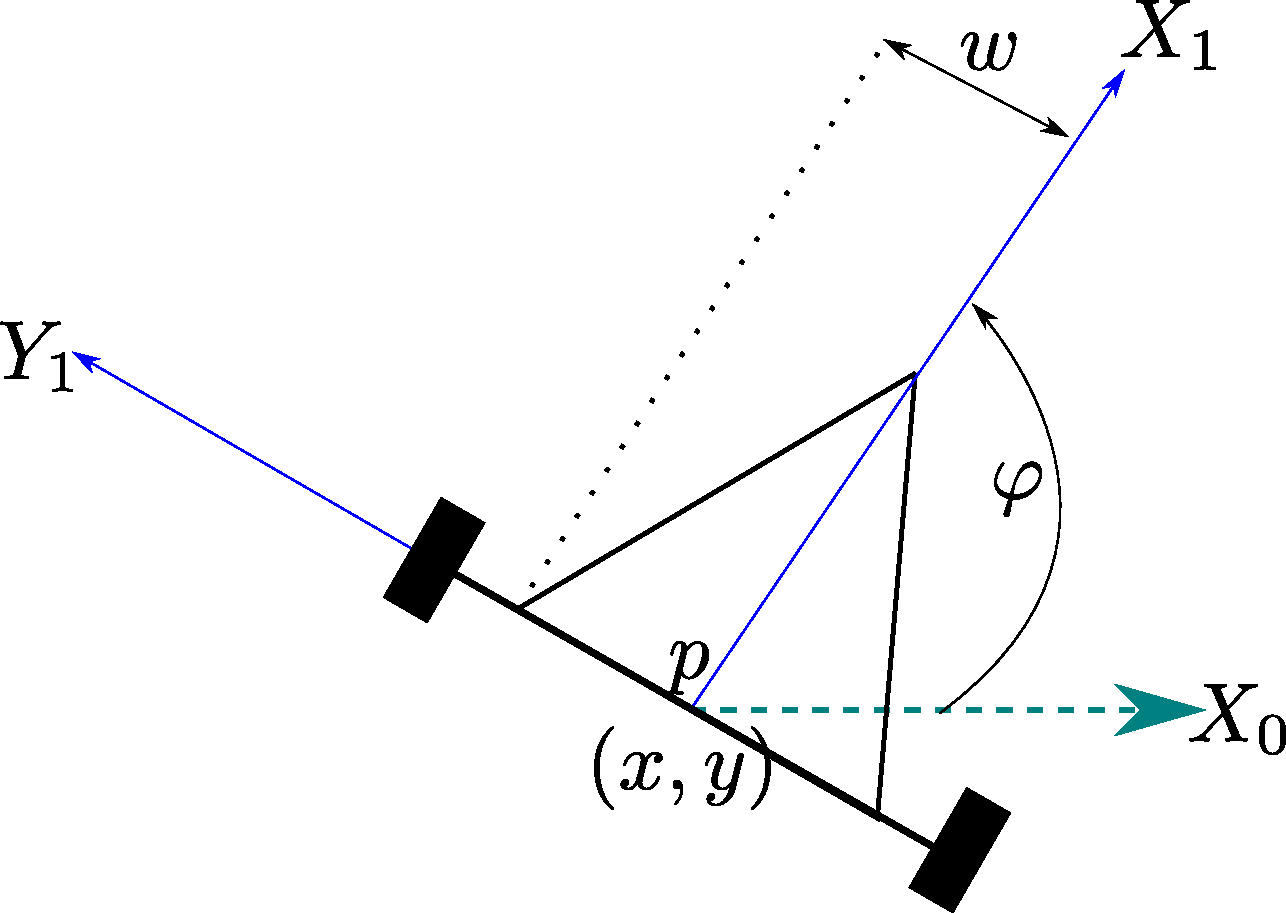
\includegraphics[width=0.5\linewidth]{Bilder/DifferentialDriveRobot.pdf}
	\caption{Differential drive robot}
	\label{Fig_DD_Robot}
\end{figure}
In deriving kinematic model, it is important to recognize the geometry of importance. In this case, the center of mass of the robot is considered. For the rotation of each wheels a scenario is considered and the kinematics of the robot is determined. For the first case, consider figure \ref{fig_2_ch_3_KD_DR_1}, where a case is considered such that $v_r \neq 0$ and $v_l = 0$, where $v_l$ and $v_r$ are the velocities of the left and right wheels respectively.
\begin{figure}[h!]
	\centering
	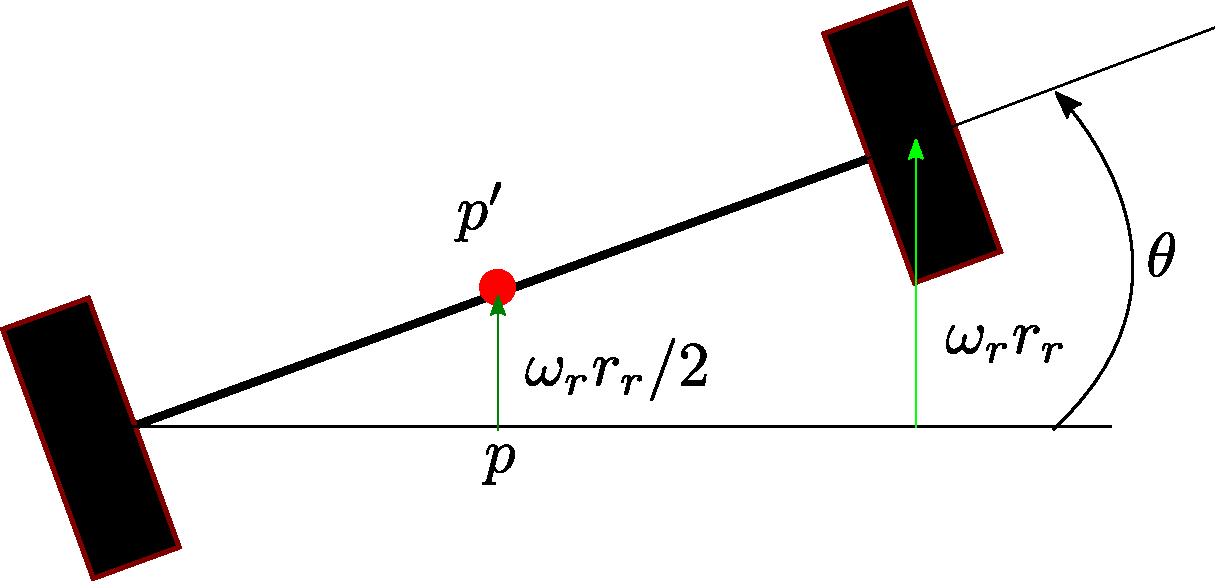
\includegraphics[width=0.4\linewidth]{Bilder/30_DifferentialRobot2.pdf}
	\caption{Kinematic configuration with $v_r \neq 0$ and $v_l = 0$}
	\label{fig_2_ch_3_KD_DR_1}
\end{figure}
with reference to figure \ref{fig_2_ch_3_KD_DR_1}, $r_r$ is the radius of the right wheel and $\omega_{r}$ is angular velocity of the robot when only $v_r \neq 0$. $p$ is the position of mass center when at rest and $p^{\prime}$ is the position with a certain $\omega_{r}$.

The distance covered by the right wheel is expressed by,
\begin{equation}
	d = \omega_{r} r_{r}
\end{equation}
therefore, the position $p^{\prime}$, can be expressed as,
\begin{equation} \label{eq_2_ch_3_DDR_VR}
\dot{p}^{\prime}_{x} = \frac{\omega_{r} r_{r}}{2}
\end{equation}
Assuming that th wheel do not slip, the velocity normal to forward direction will be zero such that $\dot{p}^{\prime}_{y} = 0$.

Additionally, using the relationship $\vec{v} = \dot{\theta} \hat{j} \times \vec{r}$, where $\vec{r}$ is the position of the displaced point from the center of rotation, the following expression for $\dot{\theta}$ can be evaluated:
\begin{equation} \label{Eq_2_ch_3_DDR_omegaR}
	\omega_{r} r_{r} = 2w \dot{\theta} \implies \dot{\theta} = \frac{\omega_{r} r_{r}}{2w}
\end{equation}
Performing same calculations as in the earlier case, this time using configuration $v_r = 0$ and $v_l \neq 0$ as shown in figure \ref{fig_2_ch_3_KD_DR_2}.
\begin{figure}[h!]
	\centering
	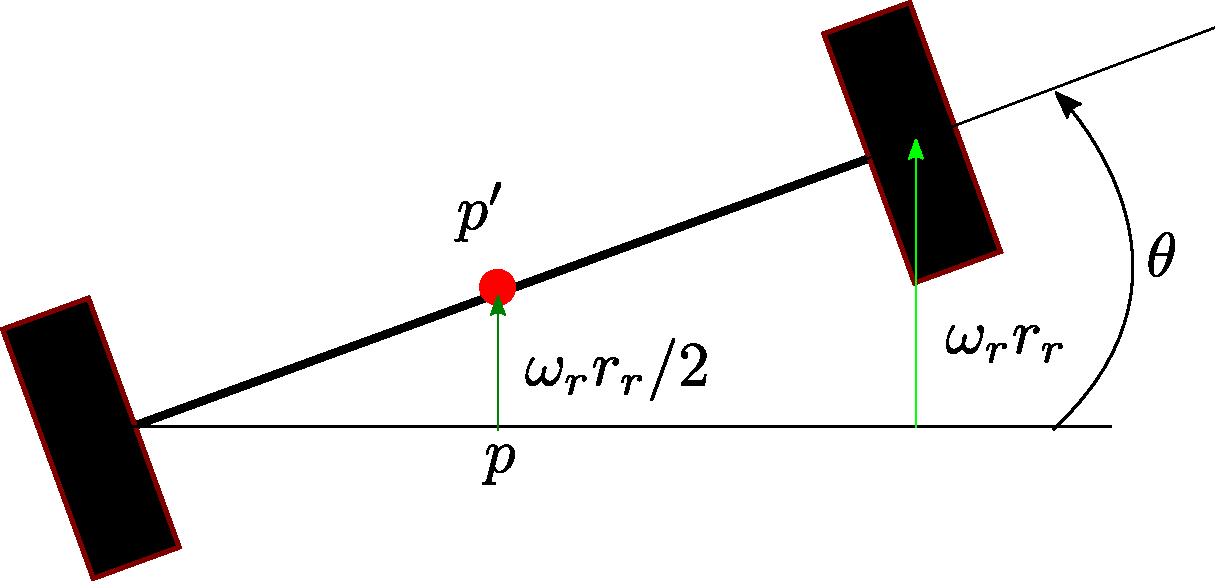
\includegraphics[width=0.4\linewidth]{Bilder/30_DifferentialRobot2.pdf}
	\caption{Kinematic configuration with $v_r = 0$ and $v_l \neq 0$}
	\label{fig_2_ch_3_KD_DR_2}
\end{figure}
The distance covered by the right wheel is expressed by,
\begin{equation}
d = \omega_{l} r_{l}
\end{equation}
therefore, the position $p^{\prime}$, can be expressed as,
\begin{equation} \label{eq_2_ch_3_DDR_VL}
\dot{p}^{\prime}_{x} = \frac{\omega_{l} r_{l}}{2}
\end{equation}
Assuming that th wheel do not slip, the velocity normal to forward direction will be zero such that $\dot{p}^{\prime}_{y} = 0$.

Additionally, using the relationship $\vec{v} = \dot{\theta} \hat{j} \times \vec{r}$, where $\vec{r}$ is the position of the displaced point from the center of rotation, the following expression for $\dot{\theta}$ can be evaluated:
\begin{equation} \label{Eq_2_ch_3_DDR_omegaL}
\omega_{l} r_{l} = - 2w \dot{\theta} \implies \dot{\theta} = - \frac{\omega_{l} r_{l}}{2w}
\end{equation}

Using equations \eqref{eq_2_ch_3_DDR_VR} and \eqref{eq_2_ch_3_DDR_VL}, since in any given case, both the velocities are non-zero, the effect of both of these can be added together. Since velocity is a vector, using vector addition, the followinf relation is determined for transnational velocity of the robots mass center,
\begin{equation} \label{eq__ch_3_DDR_EOM1}
	\vec{v} =  \frac{\omega_{l} r_{l}}{2} + \frac{\omega_{r} r_{r}}{2} = \frac{R}{2} \left(\omega_{r} + \omega_{l}\right)
\end{equation}
where $R$ is the radius of the wheels.

Similarly, angular velocity is also a vector quantity, performing vector addition for the case when both the wheel velocities are non-zero,
\begin{equation} \label{eq__ch_3_DDR_EOM2}
	\dot{\varphi} = \frac{\omega_{r} r_{r}}{2w} - \frac{\omega_{l} r_{l}}{2w} = \frac{R}{2L} \left(\omega_{r} - \omega_{l}\right)
\end{equation}
Where $L$ is replaced with $w$ and $\varphi$ is replace with $\theta$ which is in terms of notations in robotics.

Both the equations \eqref{eq__ch_3_DDR_EOM1} and \eqref{eq__ch_3_DDR_EOM2} together represent the kinematic equations for describing the motion of the differential robot.

These vector quantities can be expressed now in the global frame using the relation,
\begin{equation}\label{eq_2_ch_3_BvectorsExpInN}
	\vec{v} = \prescript{N}{}{\vec{R}_{B}} \vec{b}
\end{equation}
where
\begin{itemize}
	\item $\vec{v}$ are the vectors expressed in frame N
	\item $\vec{b}$ are the vectors expressed in frame B
	\item $\prescript{N}{}{\vec{R}_{B}}$ is the rotation matrix when B is rotated with reference to N
\end{itemize}
using equation \ref{eq_2_ch_3_BvectorsExpInN},
\begin{equation}
	\begin{bmatrix} \dot{x} \\ \dot{y} \\ \dot{\varphi} \end{bmatrix} = \begin{bmatrix}
		cos\phi & -sin\phi & 0 \\ sin\phi & cos\phi & 0 \\ 0 & 0 & 1
	\end{bmatrix} \begin{bmatrix}
		\frac{R}{2} \left(\omega_{r} + \omega_{l}\right) \\ 0 \\ \frac{R}{2L} \left(\omega_{r} - \omega_{l}\right)
	\end{bmatrix}
\end{equation}
therefore, the vectors are expressed in frame N as,
\begin{equation} \label{Eq_2_ch_3_difffDriveRobotEuqations}
		\begin{bmatrix} \dot{x} \\ \dot{y} \\ \dot{\varphi} \end{bmatrix} = \begin{bmatrix}
		\frac{R}{2} \left(\omega_{r} + \omega_{l}\right) cos\phi \\ \frac{R}{2} \left(\omega_{r} + \omega_{l}\right) sin\phi \\ \frac{R}{2L} \left(\omega_{r} - \omega_{l}\right)
		\end{bmatrix}
\end{equation}
